\documentclass[10pt,a4paper]{article}
\usepackage[T1]{fontenc}
\usepackage{lmodern}
\usepackage[margin=2.2cm]{geometry}
\usepackage{amsmath,amssymb}
\usepackage{booktabs}
\usepackage{graphicx}
\usepackage{float}
\usepackage{xcolor}
\usepackage[font=small,labelfont=bf]{caption}
\usepackage{microtype}
\usepackage{enumitem}
\usepackage{tikz}
\usetikzlibrary{arrows.meta,positioning}
\usepackage[colorlinks=true,linkcolor=blue!50!black,citecolor=blue!50!black,urlcolor=blue!50!black]{hyperref}
\setlist{itemsep=1pt,topsep=3pt}
\newcommand{\nFrel}{0.277}
\newcommand{\nSoh}{1.85}
\newcommand{\nfitrmse}{0.382}
\newcommand{\nW}{9.83}
\newcommand{\nalpha}{0.2595}
\newcommand{\nbeta}{0.0180}
\newcommand{\nmalpha}{2.2778}
\newcommand{\nmbeta}{0.1095}
\newcommand{\nkOneZero}{0.1543}
\newcommand{\nkOneTwo}{0.0930}
\newcommand{\nkTwoOne}{0.0303}
\newcommand{\nmOneZero}{2.1002}
\newcommand{\nmOneTwo}{0.1683}
\newcommand{\nmTwoOne}{0.1187}
\newcommand{\ntalpha}{2.67}
\newcommand{\ntbeta}{38.54}
\newcommand{\ntmalpha}{0.30}
\newcommand{\ntmbeta}{6.33}
\newcommand{\ntka}{0.35}
\newcommand{\nteaMGcmax}{151.9}
\newcommand{\nteaMGtmax}{1.20}
\newcommand{\nteaMGauc}{1322}
\newcommand{\nteaOHcmax}{14.5}
\newcommand{\nteaOHtmax}{1.85}
\newcommand{\nteaOHauc}{144}
\newcommand{\nRperg}{75.55}
\newcommand{\nEpeakperg}{187.68}
\newcommand{\nEtmax}{1.66}
\newcommand{\naccum}{1.145}
\newcommand{\nRpeakperg}{214.91}
\newcommand{\nsinglepeakrel}{248}
\newcommand{\nsspeakrel}{284}
\newcommand{\nshareOHauc}{66}
\newcommand{\nshareOHpeak}{63}
\newcommand{\ndirectOH}{0.19}
\newcommand{\nshapeEOne}{88}
\newcommand{\nshapeETwo}{98}
\newcommand{\nshapeEFour}{67}
\newcommand{\nshapeESix}{43}
\newcommand{\nshapeEEight}{29}
\newcommand{\nshapeEOneTwo}{15}
\newcommand{\nshapeETwoFour}{6}
\newcommand{\nshapeEFourEight}{3}
\newcommand{\nshapeESevenTwo}{2}
\newcommand{\nshapeEOneSixEight}{0}
\newcommand{\nshapeMGOne}{99}
\newcommand{\nshapeMGTwo}{91}
\newcommand{\nshapeMGFour}{58}
\newcommand{\nshapeMGSix}{37}
\newcommand{\nshapeMGEight}{24}
\newcommand{\nshapeMGOneTwo}{12}
\newcommand{\nshapeMGTwoFour}{5}
\newcommand{\nshapeMGFourEight}{3}
\newcommand{\nshapeMGSevenTwo}{2}
\newcommand{\nshapeMGOneSixEight}{0}
\newcommand{\nshapeOHOne}{80}
\newcommand{\nshapeOHTwo}{100}
\newcommand{\nshapeOHFour}{71}
\newcommand{\nshapeOHSix}{46}
\newcommand{\nshapeOHEight}{31}
\newcommand{\nshapeOHOneTwo}{16}
\newcommand{\nshapeOHTwoFour}{6}
\newcommand{\nshapeOHFourEight}{3}
\newcommand{\nshapeOHSevenTwo}{2}
\newcommand{\nshapeOHOneSixEight}{0}
\newcommand{\nwashOne}{37.5}
\newcommand{\nwashTwo}{23.3}
\newcommand{\nwashThree}{15.1}
\newcommand{\nwashSeven}{2.7}
\newcommand{\nwashOneFour}{0.1}
\newcommand{\ntailSeven}{0.38}
\newcommand{\ntailOneZero}{0.10}
\newcommand{\ntailOneFour}{0.02}
\newcommand{\nuncloOneTwo}{9}
\newcommand{\nuncmedOneTwo}{15}
\newcommand{\nunchiOneTwo}{27}
\newcommand{\nuncloTwoFour}{3}
\newcommand{\nuncmedTwoFour}{6}
\newcommand{\nunchiTwoFour}{10}
\newcommand{\tabSD}{6.65 & 17.1 & 11.9 & 52.8 & 103 & 3.6 & 2.1 & 11.2 & 21 \\
13.3 & 32.1 & 23.7 & 136 & 207 & 6.6 & 4.2 & 28.8 & 42 \\
26.6 & 57 & 47.5 & 364 & 413 & 10.8 & 8.4 & 58.2 & 83 \\
53.2 & 125 & 95.0 & 908 & 827 & 22.7 & 16.8 & 136 & 167 \\}
\newcommand{\tabMD}{6.65 & 21.4 & 13.4 & 1.4 & 1.55 & 85.1 & 103 & 3.2 & 2.4 & 10.1 & 21 \\
13.3 & 33.5 & 26.8 & 2.74 & 3.09 & 175 & 207 & 5.9 & 4.8 & 28 & 42 \\
26.6 & 74.6 & 53.5 & 7.7 & 6.19 & 457 & 413 & 11.3 & 9.6 & 67.8 & 83 \\
53.2 & 143 & 107.0 & 20.5 & 12.37 & 958 & 826 & 21.8 & 19.3 & 133 & 167 \\}
\newcommand{\tabCoef}{1 & 0.017984 & 38.54 & +0.443066 & +0.049497 & +14.56008 \\
2 & 0.109472 & 6.33 & 0 & +0.051653 & +10.04373 \\
3 & 0.259527 & 2.67 & +9.433512 & +1.005442 & +300.59118 \\
4 & 1.990000 & 0.35 & -9.876578 & -7.829166 & -1632.38407 \\
5 & 2.277782 & 0.30 & 0 & +6.722574 & +1307.18908 \\}
\newcommand{\nexMGlo}{87}\newcommand{\nexMGhi}{121}\newcommand{\nexOHlo}{3.8}\newcommand{\nexOHhi}{6.8}
\newcommand{\tabAmt}{1 & 0.017984 & +7.03624 & +0.19781 \\
2 & 0.109472 & 0 & +1.48270 \\
3 & 0.259527 & +10.38122 & -0.29434 \\
4 & 1.990000 & -17.41746 & -10.66058 \\
5 & 2.277782 & 0 & +9.27441 \\}
\newcommand{\ntbetac}{38.5}
\newcommand{\nheavyg}{12}
\newcommand{\ntfast}{20}
\newcommand{\ntslow}{60}
\newcommand{\ntslowheavy}{84}
\newcommand{\nsfast}{1.93}
\newcommand{\nsslow}{0.64}
\newcommand{\nsslowheavy}{0.46}
\newcommand{\ntailheavy}{0.45}
\newcommand{\nrgmcmax}{1.81}
\newcommand{\nrgmauc}{2.15}
\newcommand{\nrgmohcmax}{1.62}
\newcommand{\nrgmohauc}{1.86}
\newcommand{\nraucmin}{23.6}
\newcommand{\nraucmax}{31.7}
\newcommand{\tabReissig}{1 & 10 & 41.7 & 18 & 305.4 & 130 & 6.7 & 3.2 & 53.5 & 26 & 2.35 \\
3 & 31 & 118 & 55 & 784.8 & 391 & 17.8 & 9.7 & 132.9 & 78 & 2.01 \\
8 & 82 & 197.5 & 147 & 1942 & 1041 & 34 & 25.9 & 412.6 & 209 & 1.87 \\
10 & 103 & 318.1 & 184 & 3254 & 1301 & 48.4 & 32.4 & 459.1 & 261 & 2.50 \\
12 & 123 & 378.5 & 220 & 3271 & 1562 & 58.4 & 38.9 & 574.3 & 313 & 2.09 \\}
\newcommand{\tabTrak}{6.25 & 12.5 & 24 & 85 \\
6.25 & 6.25 & 13 & 45 \\
9.96 & 19.92 & 38 & 136 \\
9.96 & 9.96 & 20 & 72 \\
11.5 & 23 & 44 & 157 \\}
\newcommand{\tabSmith}{3 & 143 & 27 & 0.19 \\
4 & 161 & 31 & 0.19 \\
6 & 198 & 39 & 0.19 \\}
\newcommand{\tabKan}{KIDN01 & 32.3 & 26.9 & 29 & 41 & 66 \\
KIJC02 & 26.6 & 58.5 & 24 & 34 & 54 \\
KIDL03 & 54.1 & 222.4 & 49 & 69 & 110 \\
KIDM04 & 29.8 & 107.7 & 27 & 38 & 61 \\}
\newcommand{\tabWash}{fast end & 20 & 7\,h & 21\,h & 48\,h \\
central & 39 & 11\,h & 37\,h & 3.7\,d \\
slow end & 60 & 15\,h & 2.3\,d & 5.6\,d \\
slow end, heavy users & 84 & 20\,h & 3.1\,d & 7.7\,d \\}

\newcommand{\MG}{\mathrm{MG}}
\newcommand{\OH}{\mathrm{OH}}

\title{\textbf{Estimating mitragynine and 7-hydroxymitragynine\\exposure from self-reported kratom leaf-powder doses}\\[4pt]
\large Literature review, pharmacokinetic model, calibration and implementation specification\\for the \emph{bezKRATOMU} application}
\author{Technical report (model version 1)}
\date{6 November 2026}

\begin{document}
\maketitle

\begin{abstract}
\noindent
We describe how the \emph{bezKRATOMU} tapering application will estimate the time course of the two
principal opioid-active kratom alkaloids, mitragynine (MG) and its metabolite 7-hydroxymitragynine (7-OH),
from the doses (grams and time) that users record. Human pharmacokinetic (PK) studies published
2015--2026 are reviewed. Oral MG is absorbed rapidly ($t_{\max}\approx 1$--$1.5$\,h) and declines
bi-exponentially, with a fast distribution phase over the first $\sim$6\,h and a long terminal phase
(reported half-lives 9--68\,h depending on dose and sampling duration). 7-OH is formed from MG mainly by hepatic CYP3A4,
peaks slightly later ($t_{\max}\approx 1.5$--$2$\,h) and tracks the parent at a concentration ratio of about 0.1--0.3.
We adopt a published linked parent--metabolite two-compartment model (Notario \emph{et al.}, 2026),
recalibrate it to the largest dose-ranging study of encapsulated leaf powder (Huestis \emph{et al.}, 2024)
with two scale factors ($F_{\mathrm{rel}}=\nFrel$, $s_{\OH}=\nSoh$), and validate it against independent
steady-state data after 15 daily doses. The two analytes are combined into a single
potency-weighted index of $\mu$-opioid receptor activity, which is displayed on a relative scale
(100\,\% = the steady-state daily mean at the user's baseline daily amount). Because the model is linear,
the curve for any dosing history is an exact superposition of a five-term sum of exponentials,
whose coefficients are tabulated here. The result is a population-average estimate, not a measurement:
between-subject variability in the source studies is 5--10-fold.
\end{abstract}

\tableofcontents
\bigskip

\noindent\fbox{\parbox{\dimexpr\linewidth-2\fboxsep-2\fboxrule}{\small
\textbf{Scope and caveat.} The model estimates what an \emph{average} healthy adult's plasma concentrations would be
after the logged doses of a leaf powder containing 1.6\,\% MG. It does not measure anything, it does not predict effects,
craving or withdrawal, and it must not be used to decide when or how much to dose. It is not valid for kratom extracts or
7-OH products.}}

\section{Background pharmacology}

\paragraph{Alkaloids.} Dried \emph{Mitragyna speciosa} leaf contains dozens of indole and oxindole alkaloids. Mitragynine
is the most abundant (about 1--2\,\% of leaf mass; 1.33\,\% in the product of Huestis \emph{et al.}~\cite{huestis2024};
1.6\,\% in the product used by our users). 7-Hydroxymitragynine is present only in traces in leaf
(<0.01\,\% in~\cite{huestis2024}; 0.001\,\% in our users' product). Other alkaloids (e.g.\ speciociliatine, paynantheine,
speciogynine) reach substantial plasma levels~\cite{tanna2022} but are less characterised and are not modelled here.

\paragraph{Metabolic origin of 7-OH.} In humans, 7-OH plasma exposure after kratom is predominantly the result of
hepatic oxidation of MG by CYP3A4. Pretreatment with the selective CYP3A4 inhibitor itraconazole reduced 7-OH $C_{\max}$ by
56\,\% and AUC$_{0\text{--}72}$ by 43\,\%, while MG $C_{\max}$ rose about 1.5-fold~\cite{mongar2024}. A physiologically based
model reached the same conclusion (CYP3A4 inhibitors reduce 7-OH formation but change MG exposure little)~\cite{chiang2026}.
In mice, 7-OH formed from MG mediates a large part of MG's analgesic effect~\cite{kruegel2019}.

\paragraph{Receptor pharmacology.} Both compounds are G-protein-biased partial agonists at the human
$\mu$-opioid receptor (MOR). In a BRET G-protein activation assay, MG had $EC_{50}=339\pm178$\,nM ($E_{\max}=34$\,\%)
and 7-OH $EC_{50}=34.5\pm4.5$\,nM ($E_{\max}=47$\,\%)~\cite{kruegel2016,fda7oh}, i.e.\ 7-OH is about tenfold more potent.
Binding affinities differ between assays (7-OH $K_i$ 8--47\,nM; MG $K_i\approx 230$\,nM)~\cite{fda7oh}. MG also acts at
adrenergic and other receptors; these non-opioid actions are ignored in this report.

\paragraph{Protein binding.} Both MG and 7-OH are more than 90\,\% bound in human plasma (equilibrium dialysis)~\cite{manda2014};
reported MG binding is 85--97\,\%. As the unbound fractions are similar, we compare total concentrations.

\section{Human pharmacokinetic literature}

\begin{table}[H]\centering\small
\caption{Human PK studies used in this report. Values are means or medians as reported by the authors.
MG = mitragynine; 7-OH = 7-hydroxymitragynine; SD = single dose; MD = multiple (daily) doses.}
\label{tab:lit}
\begin{tabular}{@{}p{2.6cm}p{3.6cm}p{4.6cm}p{4.2cm}@{}}
\toprule
Study & Population and dose & Mitragynine & 7-OH \\
\midrule
Trakulsrichai 2015~\cite{trak2015} & 9 chronic male users; tea, 6.25--23\,mg MG; no washout & $t_{\max}$ 0.83\,h; $t_{1/2}$ 23.2$\pm$16.1\,h; biexponential; $C_{\max}$, AUC proportional to dose & not measured \\
Tanna 2022~\cite{tanna2022} & 5--6 healthy adults; 2\,g leaf powder as tea & $t_{\max}$ 1\,h; $t_{1/2}$ 45.3\,h (median); two-compartment model fits best & $t_{\max}$ 1\,h; $t_{1/2}$ 5.7\,h; AUC ratio to MG 0.24 \\
Mongar 2024~\cite{mongar2024} & 15--16 healthy adults; tea, 23.6\,mg MG; $\pm$ itraconazole & $C_{\max}$ 159\,ng/mL at 0.84\,h; $t_{1/2}$ 8.7\,h (72\,h sampling); biphasic & $C_{\max}$ 12.8\,ng/mL at 1.77\,h; $t_{1/2}$ 7.4\,h; CYP3A4-dependent \\
Huestis 2024~\cite{huestis2024} & 8--13 per arm, healthy adults; capsules 0.5--4\,g leaf (6.65--53.2\,mg MG); SD and 15 daily doses & $t_{\max}$ 1.0--1.3\,h; $C_{\max}$ dose-proportional; median $t_{1/2}$ 3.7$\to$42.9\,h (SD), 14.6$\to$61.2\,h (MD); steady state 8--9\,d & $t_{\max}$ 1.2--1.8\,h; $t_{1/2}$ 1.7--4.7\,h (SD); ratio to MG 0.2--0.3 (SD), 0.15--0.21 (MD) \\
Huestis 2026~\cite{huestis2026} & Extract (39.5\,\% MG), 9.9--59.2\,mg MG; SD and 15 MD & $C_{\max}$ 32.8--196\,ng/mL; $t_{\max}$ 1.3--2\,h; AUC $<1.4\times$ proportional; higher exposure than leaf & $C_{\max}$ 6.8--30.5\,ng/mL; $t_{\max}$ 1.3--2.3\,h \\
Notario 2026~\cite{notario2026} & Model fitted (Bayesian, HMC) to Mongar 2024 data & linked parent--metabolite, 2+2 compartments, first-order absorption & formation fraction $F_m=0.65$ \\
\bottomrule
\end{tabular}
\end{table}

\subsection{Absorption}
All studies agree that absorption of oral MG is fast: median $t_{\max}$ is 0.8--1.3\,h after tea or capsules and
1.3--2.0\,h at steady state or after extracts. 7-OH appears in plasma within 15\,min~\cite{mongar2024} and peaks
0.2--0.9\,h after MG, as expected for a formed metabolite. Some participants showed secondary 7-OH peaks
after a meal 4\,h post-dose~\cite{huestis2024}. Tanna \emph{et al.} noted that sparse early sampling limited the
characterisation of absorption~\cite{tanna2022}.

\subsection{Distribution and elimination}
Concentration--time profiles are bi-exponential: ``an initial rapid descent after $C_{\max}$ for about 6\,h and then a
much slower terminal phase''~\cite{huestis2024}; see also~\cite{trak2015,tanna2022,mongar2024}.
Apparent volumes are very large (MG $V_z/F$ 1\,000--13\,000\,L), consistent with extensive tissue distribution
of a lipophilic base. The terminal half-life reported for MG varies widely (8.7--68\,h). Most of this spread is methodological:
\begin{itemize}
\item \emph{Sampling duration and assay sensitivity.} The slow phase is visible only as long as concentrations stay above the
limit of quantification. Studies that sample for 72\,h~\cite{mongar2024} or give low doses report short half-lives, and studies that
sample for 5--10\,days at higher doses report long ones~\cite{huestis2024,tanna2022}. Huestis \emph{et al.} state that half-lives
``were best reflected at higher doses due to the ability to measure low analyte concentrations longer''~\cite{huestis2026}.
\item \emph{Possible saturation.} The same authors also raise possible enzyme saturation at higher doses~\cite{huestis2026}.
AUC rose slightly more than dose-proportionally (1.18--1.42-fold over the dose range)~\cite{huestis2024}.
\end{itemize}
The terminal phase carries little of the total exposure: in~\cite{huestis2024} AUC$_{0\text{--}24}$ was already
61--80\,\% of AUC$_{0\text{--}\infty}$ after one dose. Accumulation on once-daily dosing is therefore modest
(MG $C_{\max}$ ratio 1.1--1.3, AUC ratio 1.6--1.9; 7-OH 0.9--1.0 and 1.0--1.3)~\cite{huestis2024}.

\subsection{Linearity and variability}
$C_{\max}$ of both analytes increased dose-proportionally over 6.65--53.2\,mg MG, and AUC increased slightly more than
proportionally~\cite{huestis2024}; extracts gave less than $1.4\times$ the proportional increase~\cite{huestis2026}. Trakulsrichai
found linear kinetics over 6--23\,mg~\cite{trak2015}. A linear model is therefore a reasonable first approximation.
Between-subject variability is large: at 0.5\,g leaf, MG $C_{\max}$ ranged 1.8--61.5\,ng/mL; at 4\,g, 34--204\,ng/mL~\cite{huestis2024}.
Sources of variability include CYP3A4 activity~\cite{mongar2024,huestis2026}, food, and product composition.

\subsection{Formulation}
Exposure per mg of MG differs between preparations and studies: the tea of Mongar \emph{et al.} gave AUC$_{0\text{--}\infty}$
of 940\,ng\,h/mL for 23.6\,mg MG~\cite{mongar2024}, whereas 26.6\,mg in capsules gave 364\,ng\,h/mL~\cite{huestis2024}, and
extracts gave more than leaf powder~\cite{huestis2026}. Because our users take plain leaf powder, the model is calibrated to
the capsule study~\cite{huestis2024}, which used the same material.

\section{Model}

\subsection{Structure}
We adopt the linked parent--metabolite model of Notario \emph{et al.}~\cite{notario2026}, which describes both analytes with
two compartments each and first-order absorption (Figure~\ref{fig:scheme}). Two empirical scale factors adapt it from
tea to leaf powder (\S\ref{sec:calib}).

\begin{figure}[H]\centering
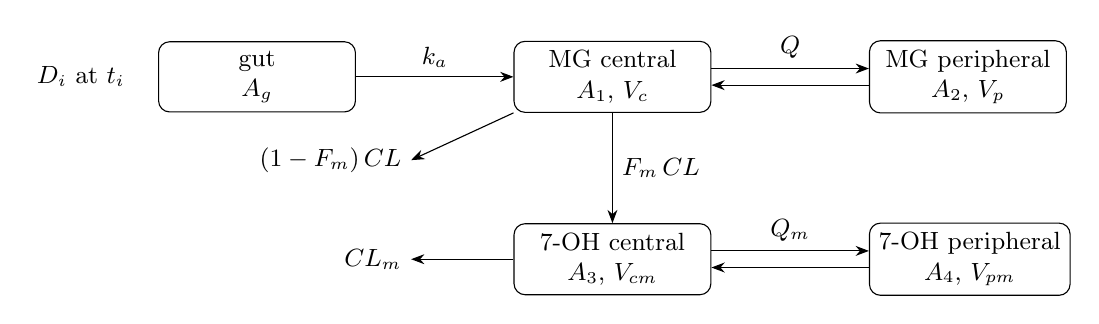
\begin{tikzpicture}[node distance=1.2cm and 2.0cm, box/.style={draw,rounded corners,minimum width=2.5cm,minimum height=0.8cm,align=center,font=\small}, >=Stealth]
\node[box] (gut) {gut\\$A_g$};
\node[box,right=of gut] (pc) {MG central\\$A_1$, $V_c$};
\node[box,right=of pc] (pp) {MG peripheral\\$A_2$, $V_p$};
\node[box,below=1.4cm of pc] (mc) {7-OH central\\$A_3$, $V_{cm}$};
\node[box,right=of mc] (mp) {7-OH peripheral\\$A_4$, $V_{pm}$};
\draw[->] (gut) -- node[above,font=\small]{$k_a$} (pc);
\draw[->] ([yshift=3pt]pc.east) -- node[above,font=\small]{$Q$} ([yshift=3pt]pp.west);
\draw[<-] ([yshift=-3pt]pc.east) -- ([yshift=-3pt]pp.west);
\draw[->] ([yshift=3pt]mc.east) -- node[above,font=\small]{$Q_m$} ([yshift=3pt]mp.west);
\draw[<-] ([yshift=-3pt]mc.east) -- ([yshift=-3pt]mp.west);
\draw[->] (pc) -- node[right,font=\small]{$F_m\,CL$} (mc);
\draw[->] (pc.south west) -- ++(-1.3,-0.6) node[left,font=\small]{$(1-F_m)\,CL$};
\draw[->] (mc.west) -- ++(-1.3,0) node[left,font=\small]{$CL_m$};
\node[font=\small,anchor=east] at ([xshift=-0.3cm]gut.west) {$D_i$ at $t_i$};
\end{tikzpicture}
\caption{Model structure. Each dose $D_i$ (mg MG) enters the gut at time $t_i$. A fraction $F_m$ of MG clearance forms 7-OH.
All parameters are apparent (divided by the unknown oral bioavailability).}
\label{fig:scheme}
\end{figure}

With amounts $A$ in $\mu$g and volumes in L (so that $A/V$ is in ng/mL), the system is
\begin{align}
\dot A_g &= -k_a A_g, \\
\dot A_1 &= k_a A_g - \frac{CL+Q}{V_c}A_1 + \frac{Q}{V_p}A_2, &
\dot A_2 &= \frac{Q}{V_c}A_1 - \frac{Q}{V_p}A_2, \\
\dot A_3 &= F_m\frac{CL}{V_c}A_1 - \frac{CL_m+Q_m}{V_{cm}}A_3 + \frac{Q_m}{V_{pm}}A_4, &
\dot A_4 &= \frac{Q_m}{V_{cm}}A_3 - \frac{Q_m}{V_{pm}}A_4,
\end{align}
with plasma concentrations $C_{\MG}=A_1/V_c$ and $C_{\OH}=s_{\OH}\,A_3/V_{cm}$. A dose of $g$ grams of powder contains $D=1000\,f_{\MG}\,g$ mg MG ($f_{\MG}=0.016$, i.e.\ 16\,mg per gram) and adds
$1000\,F_{\mathrm{rel}}\,D$ $\mu$g to $A_g$.

\begin{table}[H]\centering\small
\caption{Parameters: posterior medians of Notario \emph{et al.}~\cite{notario2026} (fitted to~\cite{mongar2024}), the scale factors
fitted here, and derived quantities.}
\label{tab:par}
\begin{tabular}{@{}lrl@{\qquad}lrl@{}}
\toprule
\multicolumn{3}{c}{Mitragynine} & \multicolumn{3}{c}{7-hydroxymitragynine} \\
\midrule
$k_a$ & 1.99 & h$^{-1}$ & $F_m$ & 0.65 & -- \\
$CL$ & 17.85 & L/h & $CL_m$ & 106.29 & L/h \\
$V_c$ & 115.71 & L & $V_{cm}$ & 50.61 & L \\
$Q$ & 10.76 & L/h & $Q_m$ & 8.52 & L/h \\
$V_p$ & 355.64 & L & $V_{pm}$ & 71.76 & L \\
\midrule
\multicolumn{3}{l}{\emph{Fitted here (leaf powder)}} & & & \\
$F_{\mathrm{rel}}$ & \nFrel & -- & $s_{\OH}$ & \nSoh & -- \\
\midrule
\multicolumn{3}{l}{\emph{Derived}} & & & \\
absorption $t_{1/2}$ & \ntka & h & & & \\
$\alpha$ ($t_{1/2,\alpha}$) & \nalpha & h$^{-1}$ (\ntalpha\,h) & $\alpha_m$ ($t_{1/2}$) & \nmalpha & h$^{-1}$ (\ntmalpha\,h) \\
$\beta$ ($t_{1/2,\beta}$) & \nbeta & h$^{-1}$ (\ntbeta\,h) & $\beta_m$ ($t_{1/2}$) & \nmbeta & h$^{-1}$ (\ntmbeta\,h) \\
\bottomrule
\end{tabular}
\end{table}

The MG disposition rate constants follow from $k_{10}=CL/V_c$, $k_{12}=Q/V_c$, $k_{21}=Q/V_p$ as
$\alpha,\beta = \tfrac12\big[(k_{10}+k_{12}+k_{21}) \pm \sqrt{(k_{10}+k_{12}+k_{21})^2-4k_{10}k_{21}}\,\big]$,
and analogously for 7-OH. The resulting MG distribution half-life of \ntalpha\,h and terminal half-life of \ntbeta\,h
agree with the ``fast fall for about 6\,h, then slow tail'' pattern and with the long half-lives reported by studies
that sampled for 5--10 days (Table~\ref{tab:lit}). 7-OH's own disposition is fast (\ntmalpha\,h and \ntmbeta\,h),
so its plasma level is \emph{formation-rate-limited}: after the first few hours it follows the MG curve with a roughly constant ratio.
The short 7-OH half-lives reported clinically (1.7--5.7\,h) reflect the fast distribution phase of the parent, as the
metabolite falls below the limit of quantification before the slow tail is reached.

\subsection{Direct 7-OH in the powder}
The users' product contains 0.001\,\% 7-OH (0.01\,mg per gram) against 16\,mg MG per gram. Even assuming complete bioavailability
of ingested 7-OH, its contribution to 7-OH exposure (same clearance $CL_m$) is at most
$0.01/(s_{\OH}\,F_{\mathrm{rel}}\,F_m\cdot 16)=\ndirectOH$\,\% of the 7-OH formed from MG. It is therefore neglected.

\subsection{Analytical solution and superposition}
The system $\dot{\mathbf A}=\mathbf K\mathbf A$ is linear and time-invariant, and $\mathbf K$ is lower block-triangular with
five distinct real eigenvalues $-\lambda_k \in \{-k_a,-\alpha,-\beta,-\alpha_m,-\beta_m\}$. The response to a unit
dose is therefore a sum of exponentials,
\begin{equation}
h_{\MG}(\tau)=\sum_{k=1}^{5} a_k e^{-\lambda_k\tau},\qquad h_{\OH}(\tau)=\sum_{k=1}^{5} b_k e^{-\lambda_k\tau},\qquad \tau\ge 0,
\end{equation}
obtained from the eigen-decomposition $\mathbf K=\mathbf V\boldsymbol\Lambda\mathbf V^{-1}$:
$\mathbf A(\tau)=\mathbf V e^{\boldsymbol\Lambda\tau}\mathbf V^{-1}\mathbf A(0)$. Here $h$ is the response to 1\,mg of MG entering the gut. For a dosing history $\{(t_i,g_i)\}$
(grams of powder at times $t_i$, i.e.\ $D_i=16\,g_i$ mg MG) the concentrations are exact superpositions,
\begin{equation}
C_{\MG}(t)=F_{\mathrm{rel}}\!\sum_{i:\,t_i\le t} D_i\, h_{\MG}(t-t_i),\qquad C_{\OH}(t)=s_{\OH}F_{\mathrm{rel}}\!\sum_{i:\,t_i\le t} D_i\, h_{\OH}(t-t_i).
\label{eq:super}
\end{equation}
No numerical integration is needed in the app; the coefficients (per gram of the users' powder, already including
$F_{\mathrm{rel}}$, $f_{\MG}$ and $s_{\OH}$ for $c_k$ below) are listed in Table~\ref{tab:coef}. The coefficients of each analyte sum to
zero, so $h(0)=0$.

\section{Calibration and validation}\label{sec:calib}

\subsection{Procedure}
The Notario parameters reproduce the tea study they were fitted to (model vs.\ observed~\cite{mongar2024}: MG $C_{\max}$ \nteaMGcmax{}
vs.\ 159\,ng/mL, $t_{\max}$ \nteaMGtmax{} vs.\ 0.84\,h; 7-OH $C_{\max}$ \nteaOHcmax{} vs.\ 12.8\,ng/mL, $t_{\max}$ \nteaOHtmax{} vs.\ 1.77\,h).
For leaf-powder capsules, exposure per mg MG is lower and the 7-OH:MG ratio is higher (Table~\ref{tab:lit}). We therefore estimated
a relative apparent bioavailability $F_{\mathrm{rel}}$ (scaling both analytes) and a metabolite scale $s_{\OH}$ (scaling 7-OH only)
by least squares on the log scale, using the 16 single-dose mean values of Huestis \emph{et al.}~\cite{huestis2024}
($C_{\max}$ and AUC$_{0\text{--}\infty}$ of both analytes at four doses). The time-course parameters were not refitted.
$F_{\mathrm{rel}}$ absorbs everything that makes the capsule cohort's exposure per mg lower than the tea cohort's
(formulation, population, assay), and $s_{\OH}$ absorbs the higher metabolite ratio. Neither has a mechanistic interpretation.

Result: $F_{\mathrm{rel}}=\nFrel$, $s_{\OH}=\nSoh$, root-mean-square log error $\nfitrmse$ (a typical deviation of
$\times$\,$e^{\nfitrmse}$). The residual pattern is systematic (Table~\ref{tab:sd}). (i) Peaks are 17--30\,\% lower than observed at every dose, i.e.\ the
tea-derived time course is slightly flatter than the capsule data. (ii) AUC is over-predicted at low doses (about $2\times$ at 6.65\,mg)
and slightly under-predicted at 53.2\,mg, because observed AUC grows more than proportionally with dose while a linear model
cannot. Both deviations are well within the between-subject range of the data.

\begin{table}[H]\centering\small
\caption{Calibration: single dose, observed (means, Huestis 2024~\cite{huestis2024}) vs.\ model. $C_{\max}$ in ng/mL; AUC$_{0\text{--}\infty}$ in ng\,h/mL.}
\label{tab:sd}
\begin{tabular}{@{}r rr rr rr rr@{}}
\toprule
 & \multicolumn{2}{c}{MG $C_{\max}$} & \multicolumn{2}{c}{MG AUC} & \multicolumn{2}{c}{7-OH $C_{\max}$} & \multicolumn{2}{c}{7-OH AUC} \\
\cmidrule(lr){2-3}\cmidrule(lr){4-5}\cmidrule(lr){6-7}\cmidrule(lr){8-9}
mg MG & obs & model & obs & model & obs & model & obs & model \\
\midrule
\tabSD
\bottomrule
\end{tabular}
\end{table}

\subsection{Validation against repeated dosing}
The calibrated model was then used to predict day 15 of once-daily dosing, data not used in the fit (Table~\ref{tab:md},
Figure~\ref{fig:calib}b). Peaks and AUCs are predicted within a factor of about 2 (the largest deviation is the 7-OH AUC at the lowest dose),
and MG troughs within 20\,\% at the three lower doses. At 53.2\,mg the trough is under-predicted (12.4 vs.\ 20.5\,ng/mL), consistent with the longer
half-life observed at high doses. The model reproduces the modest observed accumulation: the steady-state peak of the combined index is
\naccum{} times the single-dose peak (observed MG $C_{\max}$ ratio 1.1--1.3).

\begin{table}[H]\centering\small
\caption{Validation: day 15 of daily dosing, observed (means~\cite{huestis2024}) vs.\ model. Trough = concentration 24\,h after the 15th dose.}
\label{tab:md}
\begin{tabular}{@{}r rr rr rr rr rr@{}}
\toprule
 & \multicolumn{2}{c}{MG $C_{\max,ss}$} & \multicolumn{2}{c}{MG trough} & \multicolumn{2}{c}{MG AUC$_\tau$} & \multicolumn{2}{c}{7-OH $C_{\max,ss}$} & \multicolumn{2}{c}{7-OH AUC$_\tau$} \\
\cmidrule(lr){2-3}\cmidrule(lr){4-5}\cmidrule(lr){6-7}\cmidrule(lr){8-9}\cmidrule(lr){10-11}
mg MG & obs & model & obs & model & obs & model & obs & model & obs & model \\
\midrule
\tabMD
\bottomrule
\end{tabular}
\end{table}

\begin{figure}[H]\centering
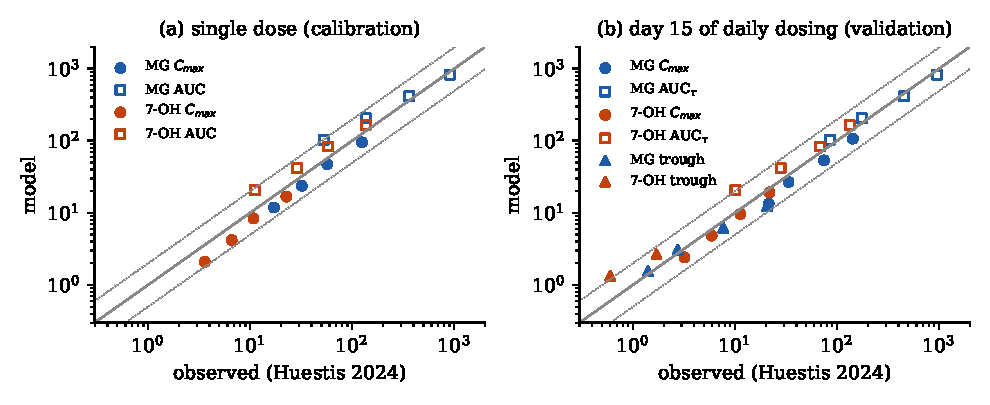
\includegraphics[width=\linewidth]{fig/calibration.pdf}
\caption{Observed vs.\ model. (a) Single doses (calibration data). (b) Day 15 of daily dosing (validation, not fitted).
Solid line: identity; dotted lines: factor 2.}
\label{fig:calib}
\end{figure}

\section{A combined activity index}

The app shows one combined line rather than two concentrations. We define a potency-weighted MOR-equivalent concentration
\begin{equation}
E(t)=\frac{C_{\MG}(t)}{M_{\MG}}+w\,\frac{C_{\OH}(t)}{M_{\OH}}\quad[\mathrm{nM}],\qquad
w=\frac{EC_{50,\MG}}{EC_{50,\OH}}=\frac{339}{34.5}=\nW,
\end{equation}
with molar masses $M_{\MG}=398.5$ and $M_{\OH}=414.5$\,g/mol (concentrations in ng/mL $\times 1000/M$ give nM). $E$ is the
MG concentration that would give the same receptor stimulation in the low-occupancy (linear) range.
Underlying assumptions: (i) equal unbound fractions ($>$90\,\% bound for both~\cite{manda2014}); (ii) equal access to the
receptor compartment (brain distribution kinetics are not modelled); (iii) potency ratio from one \emph{in vitro} assay~\cite{kruegel2016};
(iv) the difference in $E_{\max}$ (34 vs.\ 47\,\%) and receptor saturation are ignored; (v) non-opioid targets are ignored.

With $w=\nW$, 7-OH accounts for \nshareOHauc\,\% of the area under $E$ after a single dose (\nshareOHpeak\,\% at the peak),
in line with the finding that formed 7-OH mediates much of MG's opioid effect~\cite{kruegel2019}. Because 7-OH follows the MG
curve closely (formation-limited), the \emph{shape} of $E$ is insensitive to $w$ (Figure~\ref{fig:sens}a): it differs from MG alone mainly by a
slightly later peak.

\section{Relative scale shown to the user}

Absolute concentrations are not shown. The displayed level is
\begin{equation}
L(t)=100\,\frac{E(t)}{R\cdot G_0}\ \ [\%],
\end{equation}
where $G_0$ is the user's plan baseline (g/day, field \texttt{baselineG}) and $R=\nRperg$\,nM per g/day is the steady-state
\emph{daily mean} of $E$ when 1\,g/day is taken. Because the model is linear, the steady-state mean depends only on the daily amount,
not on how it is split ($\bar E = \tfrac{1}{24}\,G_0\int_0^\infty h_E\,d\tau = \tfrac{G_0}{24}\sum_k c_k/\lambda_k$). Hence
\textbf{100\,\% is the average level at the start of the taper}, and a plan that halves the daily amount brings the daily
mean to 50\,\%. Peaks rise above 100\,\%: a single baseline-sized dose from a drug-free state peaks at \nsinglepeakrel\,\%, and
taking the whole baseline once daily at steady state gives peaks of \nsspeakrel\,\% (accumulation factor \naccum). Splitting the
amount into several doses gives lower peaks (Figure~\ref{fig:dose}b).

\begin{table}[H]\centering\small
\caption{Model time course after a single dose, as \% of each curve's own peak.}
\label{tab:shape}
\begin{tabular}{@{}lrrrrrrrrrr@{}}
\toprule
hours after dose & 1 & 2 & 4 & 6 & 8 & 12 & 24 & 48 & 72 & 168 \\
\midrule
MG & \nshapeMGOne & \nshapeMGTwo & \nshapeMGFour & \nshapeMGSix & \nshapeMGEight & \nshapeMGOneTwo & \nshapeMGTwoFour & \nshapeMGFourEight & \nshapeMGSevenTwo & \nshapeMGOneSixEight \\
7-OH & \nshapeOHOne & \nshapeOHTwo & \nshapeOHFour & \nshapeOHSix & \nshapeOHEight & \nshapeOHOneTwo & \nshapeOHTwoFour & \nshapeOHFourEight & \nshapeOHSevenTwo & \nshapeOHOneSixEight \\
combined $E$ & \nshapeEOne & \nshapeETwo & \nshapeEFour & \nshapeESix & \nshapeEEight & \nshapeEOneTwo & \nshapeETwoFour & \nshapeEFourEight & \nshapeESevenTwo & \nshapeEOneSixEight \\
\bottomrule
\end{tabular}
\end{table}

After stopping from steady state (baseline taken once daily), $L$ falls to \nwashOne\,\% one day after the last dose,
\nwashTwo\,\% after 2 days, \nwashThree\,\% after 3 days, \nwashSeven\,\% after 7 days and \nwashOneFour\,\% after 14 days (measured from the last dose, as \% of the baseline daily mean).
A dose 7 days old contributes \ntailSeven\,\% of its peak and a dose 14 days old \ntailOneFour\,\%, so the app only needs
the last 14 days of doses.

\section{Amount remaining in the body}\label{sec:amount}

Alongside the relative level, the app shows how many milligrams of each analyte are still in the body. The model parameters are
\emph{apparent} (divided by the unknown absolute oral bioavailability $F$; no intravenous human data exist), so true amounts cannot
be computed. We therefore report the \emph{dose-equivalent amount not yet eliminated}, i.e.\ the amounts the model holds when the
whole ingested dose is treated as absorbed ($F_{\mathrm{rel}}$ not applied):
\begin{equation}
M_{\MG}(t)=\sum_i D_i\,\big[A_1+A_2\big]_{\text{unit}}(t-t_i),\qquad
M_{\OH}(t)=s_{\OH}\sum_i D_i\,\big[A_3+A_4\big]_{\text{unit}}(t-t_i),
\end{equation}
where $[\cdot]_{\text{unit}}$ is the response to 1\,mg in the gut. Unabsorbed drug in the gut is not counted. This is an \emph{upper
estimate} of the amount actually in the body, and it is the natural reading of ``how much of what I took is still in me''.
Because most MG resides in the peripheral compartment ($V_p\approx 3V_c$), $M_{\MG}$ changes much more smoothly than
plasma concentration. Example (70\,kg adult, the population of the calibration studies; 6\,g/day in three doses, day 14):
$M_{\MG}$ ranges \nexMGlo--\nexMGhi\,mg and $M_{\OH}$ \nexOHlo--\nexOHhi\,mg over the day, against 96\,mg MG ingested per day.
The model is not scaled for body weight. Coefficients are listed in Table~\ref{tab:amt}.

\begin{table}[H]\centering\small
\caption{Coefficients for the amounts still in the body, $M(\tau)=\sum_k d_k e^{-\lambda_k\tau}$, in mg per gram of the users' powder.}
\label{tab:amt}
\begin{tabular}{@{}crrr@{}}
\toprule
$k$ & $\lambda_k$ (h$^{-1}$) & $d_k$ MG (mg/g) & $d_k$ 7-OH (mg/g) \\
\midrule
\tabAmt
\bottomrule
\end{tabular}
\end{table}

\section{Model behaviour}

\begin{figure}[H]\centering
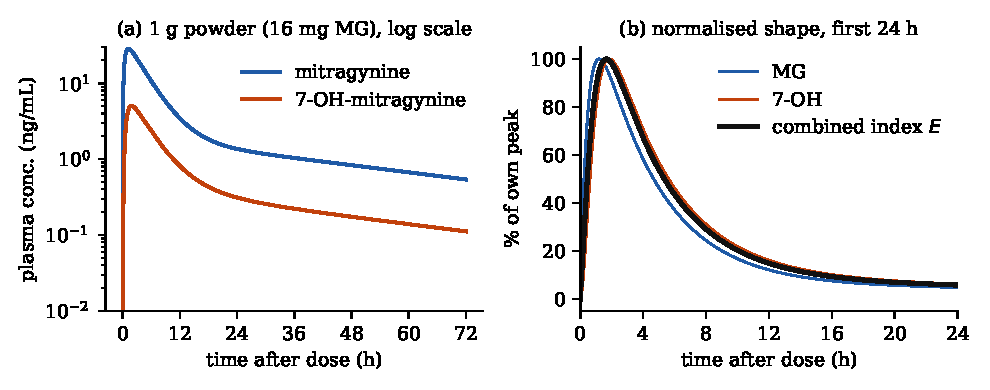
\includegraphics[width=\linewidth]{fig/single_dose.pdf}
\caption{Single dose of 1\,g powder (16\,mg MG). (a) Absolute model concentrations, log scale: fast distribution phase,
then a terminal phase with $t_{1/2}\approx\ntbeta$\,h; 7-OH runs parallel to MG. (b) Normalised shapes over 24\,h.}
\label{fig:single}
\end{figure}

\begin{figure}[H]\centering
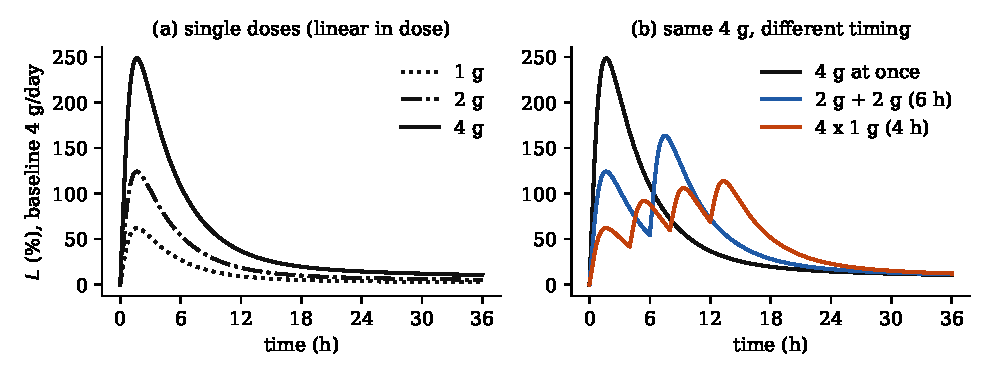
\includegraphics[width=\linewidth]{fig/dose_timing.pdf}
\caption{Dose and timing responsiveness, shown as $L$ for a user with baseline $G_0=4$\,g/day. (a) Peaks scale linearly with dose.
(b) The same daily amount split into more doses gives a lower, broader curve.}
\label{fig:dose}
\end{figure}

\begin{figure}[H]\centering
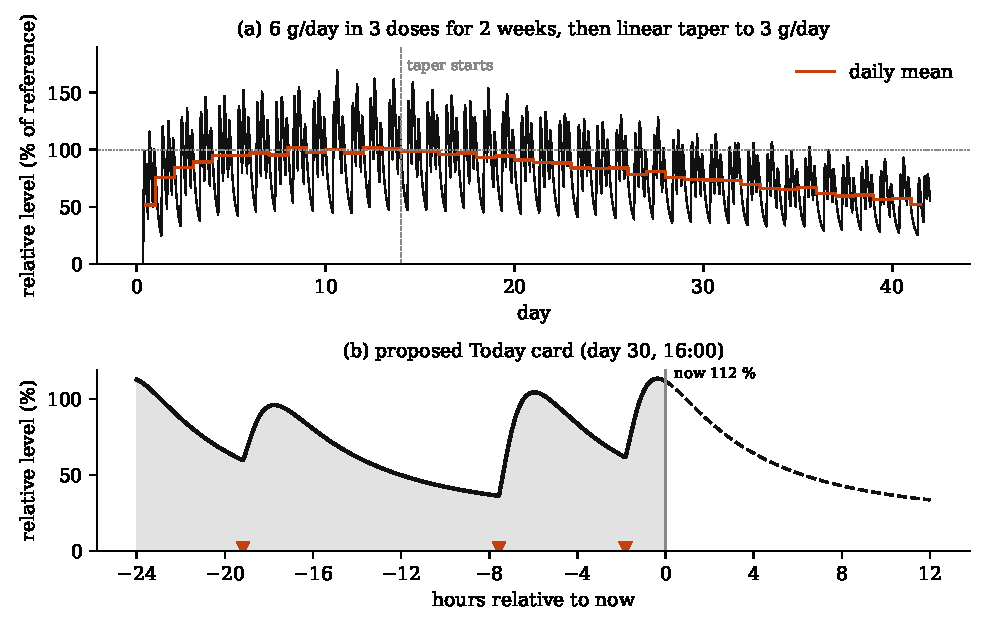
\includegraphics[width=\linewidth]{fig/taper.pdf}
\caption{Simulated user (illustrative, random dose times): baseline 6\,g/day in three doses for two weeks, then a linear
taper to 3\,g/day. (a) $L(t)$ over six weeks and its daily mean, which starts at 100\,\% and ends near 50\,\%. (b) The proposed ``Today'' card: last 24\,h (solid),
the moment ``now'', and the projection if no further dose is taken (dashed); triangles mark doses.}
\label{fig:taper}
\end{figure}

\section{Uncertainty and limitations}

\begin{figure}[H]\centering
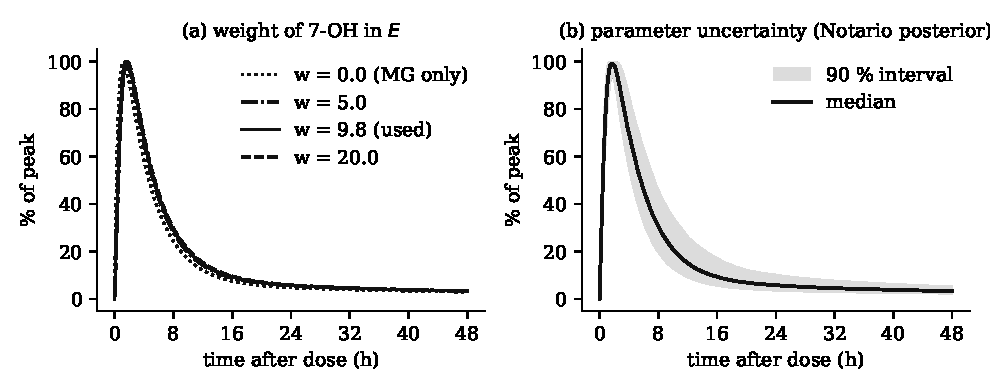
\includegraphics[width=\linewidth]{fig/sensitivity.pdf}
\caption{(a) Shape of $E$ for different 7-OH weights $w$. (b) Uncertainty of the population-average shape from the
parameter posterior (log-normal approximation of~\cite{notario2026}, 400 draws). At 12\,h the level is \nuncmedOneTwo\,\%
of peak (90\,\% interval \nuncloOneTwo--\nunchiOneTwo\,\%), at 24\,h \nuncmedTwoFour\,\% (\nuncloTwoFour--\nunchiTwoFour\,\%).}
\label{fig:sens}
\end{figure}

\begin{enumerate}
\item \textbf{Population average, not the individual.} Between-subject variability in exposure is 5--10-fold~\cite{huestis2024}
and is not represented. Figure~\ref{fig:sens}b shows only the uncertainty of the \emph{average} curve. Normalising to the user's own
baseline removes the overall scale, but not individual differences in shape (e.g.\ CYP3A4 activity).
\item \textbf{Linearity.} AUC rises up to $\sim$1.4$\times$ faster than dose~\cite{huestis2024,huestis2026}, and the high-dose trough is
under-predicted (Table~\ref{tab:md}). The relative display slightly understates how much a large dose adds compared with a small one.
\item \textbf{Calibration source.} One capsule study, with fasting. Our users' preparation (toss-and-wash, with or without food) may
absorb differently. Food delays absorption and can cause secondary peaks~\cite{huestis2024}.
\item \textbf{Chronic use.} Most participants were healthy adults, not daily long-term users. In chronic users, Trakulsrichai
reported $t_{1/2}\approx 23$\,h~\cite{trak2015}, within the range modelled.
\item \textbf{Product composition.} 1.6\,\% MG is taken as fixed; real batches vary. Other alkaloids are ignored.
\item \textbf{Interactions.} CYP3A4 inhibitors (e.g.\ itraconazole, clarithromycin, grapefruit) lower 7-OH and raise MG~\cite{mongar2024};
inducers (e.g.\ rifampicin, St John's wort) are expected to do the opposite. Not modelled.
\item \textbf{Concentration is not effect.} Tolerance, receptor adaptation and withdrawal are not modelled; withdrawal symptoms do
not map onto a plasma level. A low displayed level does not mean that a dose is needed.
\item \textbf{Not applicable} to extracts (higher exposure per mg~\cite{huestis2026}) or to semi-synthetic 7-OH products.
\end{enumerate}

\section{Implementation specification}

\begin{table}[H]\centering\small
\caption{Closed-form coefficients for $h(\tau)=\sum_k \mathrm{coef}_k\,e^{-\lambda_k\tau}$ ($\tau$ in h).
$a_k$: MG in ng/mL per mg MG reaching the gut (multiply by $16\,F_{\mathrm{rel}}$ per gram);
$b_k$: 7-OH (unscaled) likewise; $c_k$: combined index $E$ in nM per gram of the users' powder (all factors included).}
\label{tab:coef}
\begin{tabular}{@{}crrrrr@{}}
\toprule
$k$ & $\lambda_k$ (h$^{-1}$) & $t_{1/2,k}$ (h) & $a_k$ & $b_k$ & $c_k$ \\
\midrule
\tabCoef
\bottomrule
\end{tabular}
\end{table}

\begin{enumerate}
\item \textbf{Module} \texttt{src/lib/pk.ts}: constants $\lambda_k$, $c_k$, $R$ and the amount coefficients of
Table~\ref{tab:amt} (copied from \texttt{ts\_constants.json}); a pure function \texttt{level(doses, t, baselineG)} implementing $L(t)=100\sum_i g_i\sum_k c_k e^{-\lambda_k(t-t_i)}/(R\,G_0)$ (with $R=\nRperg$) over doses with
$0\le t-t_i\le 14$\,d, and a helper that returns a series on a 10-min grid for charting.
\item \textbf{Data.} The user's own doses for the last 14 days (\texttt{takenAt}, \texttt{grams}) and the plan's \texttt{baselineG}.
Runs entirely in the browser; no database change. Other users' curves are never computed (their dose times are private).
\item \textbf{Today card} (below the list of today's doses). Milligrams of MG and 7-OH still in the body (\S\ref{sec:amount}),
current $L$ (rounded to 5\,\%; it can exceed 100\,\% shortly after a dose), a 24\,h history, dose markers and a dashed 12\,h
projection with no further doses. Without an active plan there is no baseline, so the card shows the amounts and the curve
without a percentage scale. Doses logged at a later time today appear when their time comes.
\item \textbf{Tests} (\texttt{pk.test.ts}): (i) the sums of exponentials agree with a numerical ODE solution; (ii) the single-dose and
day-15 values in Tables~\ref{tab:sd} and~\ref{tab:md}; (iii) superposition and linearity; (iv) the daily mean of $L$ is 100\,\% at steady state on the baseline amount, however it is split.
\item \textbf{Wording.} Always labelled as a rough population-average estimate, not a measurement, and with no advice derived from it.
\end{enumerate}

\section*{Reproducibility}
All numbers, tables and figures in this report are generated by \texttt{docs/pk-model/model.py} (NumPy, SciPy, Matplotlib),
which writes \texttt{numbers.tex}, \texttt{numbers.json} and \texttt{fig/*.pdf}.

\begin{thebibliography}{99}\small
\bibitem{huestis2024} Huestis MA, Brett MA, Bothmer J, Atallah R. Human mitragynine and 7-hydroxymitragynine pharmacokinetics after
single and multiple daily doses of oral encapsulated dried kratom leaf powder. \emph{Molecules} 2024;29(5):984.
\href{https://doi.org/10.3390/molecules29050984}{doi:10.3390/molecules29050984}
\bibitem{huestis2026} Huestis MA, Brett MA, Bothmer J, Henningfield JE, Swift S. Mitragynine and 7-hydroxy-mitragynine plasma
pharmacokinetics in humans after single and 15 multiple oral kratom extract doses. \emph{J Anal Toxicol} 2026;50(6).
\href{https://doi.org/10.1093/jat/bkag042}{doi:10.1093/jat/bkag042} (abstract only consulted; authors compensated by an industry sponsor)
\bibitem{tanna2022} Tanna RS, Nguyen JT, Hadi DL, \emph{et al.} Clinical pharmacokinetic assessment of kratom (\emph{Mitragyna speciosa}),
a botanical product with opioid-like effects, in healthy adult participants. \emph{Pharmaceutics} 2022;14(3):620.
\href{https://doi.org/10.3390/pharmaceutics14030620}{doi:10.3390/pharmaceutics14030620}
\bibitem{mongar2024} Mongar P, Jaisi A, Inkviya T, Wungsintaweekul J, Wiwattanawongsa K. Effects of itraconazole on pharmacokinetics of
mitragynine and 7-hydroxymitragynine in healthy volunteers. \emph{ACS Pharmacol Transl Sci} 2024;7(3):823--833.
\href{https://doi.org/10.1021/acsptsci.3c00335}{doi:10.1021/acsptsci.3c00335}
\bibitem{trak2015} Trakulsrichai S, Sathirakul K, Auparakkitanon S, \emph{et al.} Pharmacokinetics of mitragynine in man.
\emph{Drug Des Devel Ther} 2015;9:2421--2429. \href{https://doi.org/10.2147/DDDT.S79658}{doi:10.2147/DDDT.S79658}
\bibitem{notario2026} Notario D, Gunawan U, Kambira PFA, Wulandari E, Prasetyanto EA. Bayesian inference for integrated pharmacokinetic
modelling of mitragynine and 7-hydroxymitragynine. \emph{ADMET DMPK} 2026;14:3170.
\href{https://doi.org/10.5599/admet.3170}{doi:10.5599/admet.3170}
\bibitem{chiang2026} Chiang Y-H, Kanumuri SRR, Berthold EC, \emph{et al.} Physiologically based pharmacokinetic model for clinical
translation and prediction of drug interaction of the major kratom alkaloid, mitragynine. \emph{ACS Pharmacol Transl Sci} 2026;9(3):620--635.
\href{https://doi.org/10.1021/acsptsci.5c00718}{doi:10.1021/acsptsci.5c00718} (abstract only consulted)
\bibitem{kruegel2016} Kruegel AC, Gassaway MM, Kapoor A, \emph{et al.} Synthetic and receptor signaling explorations of the
\emph{Mitragyna} alkaloids: mitragynine as an atypical molecular framework for opioid receptor modulators.
\emph{J Am Chem Soc} 2016;138:6754--6764. (values as quoted in~\cite{kruegel2019,fda7oh})
\bibitem{kruegel2019} Kruegel AC, Uprety R, Grinnell SG, \emph{et al.} 7-Hydroxymitragynine is an active metabolite of mitragynine
and a key mediator of its analgesic effects. \emph{ACS Cent Sci} 2019;5:992--1001.
\bibitem{fda7oh} U.S.\ Food and Drug Administration. 7-Hydroxymitragynine (7-OH): an assessment of the scientific data and
toxicological concerns around an emerging opioid threat. 2025.
\bibitem{manda2014} Manda VK, Avula B, Ali Z, \emph{et al.} Evaluation of \emph{in vitro} absorption, distribution, metabolism, and
excretion (ADME) properties of mitragynine, 7-hydroxymitragynine, and mitraphylline. \emph{Planta Med} 2014;80:568--576.
\end{thebibliography}

\end{document}
